\documentclass[final,3p,times,onecolumn]{elsarticle}
\usepackage{graphicx}
\usepackage[export]{adjustbox}
\usepackage{float}
\usepackage{paralist}
\usepackage{multirow}
\usepackage[ruled,vlined]{algorithm2e}
\usepackage{pifont}
\usepackage{textcomp}
\usepackage{comment}
\usepackage{amsmath}
\usepackage{amssymb}
\usepackage[hang,flushmargin]{footmisc}
\usepackage[utf8]{inputenc}
\AtBeginDocument{\renewcommand{\bibname}{References}}
%\usepackage[square,sort,comma,numbers,sectionbib]{natbib}
%%\usepackage{cite}
\usepackage{color}
\newcommand{\figref}[1]{\figurename~\ref{#1}}
\newcommand\addtag{\refstepcounter{equation}\tag{\theequation}}
\newcommand{\cmark}{\ding{51}}
\newcommand\aug{\fboxsep=-\fboxrule\!\!\!\fbox{\strut}\!\!\!}

\journal{Applied Soft Computing}\usepackage[T1]{fontenc}
\usepackage[utf8]{inputenc}
\usepackage{comment}
\usepackage{booktabs}
\usepackage{xargs}
\usepackage[pdftex,dvipsnames]{xcolor}
\usepackage[colorinlistoftodos,prependcaption,textsize=tiny]{todonotes}
\usepackage{tikz}
\usepackage{tabularx}

\newcommandx{\unsure}[2][1=]{\todo[linecolor=red,backgroundcolor=red!25,bordercolor=red,#1]{#2}}
\newcommandx{\change}[2][1=]{\todo[linecolor=blue,backgroundcolor=blue!25,bordercolor=blue,#1]{#2}}
\newcommandx{\info}[2][1=]{\todo[linecolor=OliveGreen,backgroundcolor=OliveGreen!25,bordercolor=OliveGreen,#1]{#2}}
\newcommandx{\improvement}[2][1=]{\todo[linecolor=Plum,backgroundcolor=Plum!25,bordercolor=Plum,#1]{#2}}
\newcommandx{\thiswillnotshow}[2][1=]{\todo[disable,#1]{#2}}
\usepackage{graphicx}
\usepackage{booktabs}
\usepackage{multirow}
\usepackage{siunitx}
\usepackage{url}
\usepackage{etoolbox}
\usepackage{algpseudocode}
\usepackage{algorithm}
\usepackage{placeins}
\newcolumntype{C}[1]{>{\centering\let\newline\\\arraybackslash\hspace{0pt}}m{#1}}

\newcolumntype{C}{>{\centering\arraybackslash}X}
\newcolumntype{R}{>{\raggedleft\arraybackslash}X}
\newcolumntype{L}{>{\raggedright\arraybackslash}X}


% Definitions of handy macros can go here

\newcommand{\dataset}{{\cal D}}
\newcommand{\fracpartial}[2]{\frac{\partial #1}{\partial  #2}}

% Heading arguments are {volume}{year}{pages}{submitted}{published}{author-full-names}


\begin{document}

\section{Experimental studies illustrating improper use of evaluation methodology}

This section aims to show the chosen flaws of commonly used experimental protocols,
i.e., how their improper use can dramatically change the results of classifier comparison.
In the first experiment, we will focus on the dataset shift problem in cross-validation while in the second, we show the problems with mean-ranks in Friedman test.


\subsection{Problems with dataset shift in cross-validation}

In this section, we will describe the details of the conducted experimental study to illustrate how partitioning methods in cross-validation, the commonly used metric estimation method, introduce dataset shift (here, strictly the covariate shift) and show its impact on the classifier comparison results.


We want to show that:

\begin{quote}
\noindent {\it Depending on the choice of the dataset folds in cross-validation, one can change the result of comparing performances of the particular two classifiers.
}
\end{quote}

Both the source code used to conduct the described experiment as well as a report with all the results are available in public Git repository\footnote{\url{https://github.com/w4k2/fair-evaluation}}. %A single instance of the problem under consideration is a typical classification experiment employing 5-fold cross-validation in the data division, whose aim is to compare the quality of two classifiers according to the basic accuracy metric. To assess the statistical significance of differences between the achieved accuracies, the \emph{t test for repeated cross-validation} is used, taking the significance level $\alpha=0.05$.

Eighteen popular datasets from \emph{\textsc{uci} Machine Learning Repository} (see Table \ref{tab:pdatasets}) \cite{Dua:2019} and three classifiers (as implemented in the \textsc{scikit-learn} library and with default parameters) % were adopted for the set of problems being the basis for the experiments, and the research itself was carried out comparing, on a peer-to-peer basis, three classifiers, according to their implementations included in the \textsc{scikit-learn} library and assuming their default parameters:

\begin{itemize}
	\item \textsc{gnb} --- Gaussian Naive Bayes,
	\item \textsc{knn} --- k-Nearest Neighbors,
	\item \textsc{dtc} --- \textsc{cart} decision tree.
\end{itemize}

were adopted for the described experimental study.


\begin{table}[!htb]
    \centering
    \caption{Overview od datasets applied in tests for Section 3.1.}
    \label{tab:pdatasets}
    \begin{adjustbox}{angle=0}
    \footnotesize

  \begin{tikzpicture}
  \node (thetable) [inner sep=0pt] {
    \begin{tabularx}{.3\textwidth}{@{}lRRR@{}}

        \toprule
        \textsc{dataset} & \textsc{samples} & \textsc{features} & \textsc{classes} \\\midrule
         \emph{breastcan} & 683 & 9 & 2 \\
\emph{wisconsin} & 699 & 9 & 2 \\
\emph{ionosphere} & 351 & 34 & 2 \\
\emph{sonar} & 208 & 60 & 2 \\
\emph{balance} & 625 & 4 & 3 \\
\emph{monkone} & 556 & 6 & 2 \\
\emph{heart} & 270 & 13 & 2 \\
\emph{liver} & 345 & 6 & 2 \\
\emph{hayes} & 160 & 4 & 3 \\
\emph{german} & 1000 & 24 & 2 \\
\emph{iris} & 150 & 4 & 3 \\
\emph{monktwo} & 601 & 6 & 2 \\
\emph{wine} & 178 & 13 & 3 \\
\emph{yeast3} & 1484 & 8 & 2 \\
\emph{monkthree} & 554 & 6 & 2 \\

         \bottomrule
    \end{tabularx}};


  \end{tikzpicture}
    \end{adjustbox}
\end{table}

For each dataset, 100 000 partitionings into 5 folds with standard stratification were performed each one being the basis for the comparison of performance of 3 classifier pairs (constructed from the above mentioned). Thus, there were 45 different classifier comparisons (18 datasets with 3 pairs of classifiers). Classifier performance was measured by the described accuracy metric (i.e. the ratio of properly classified to all elements in a test set) estimated using standard stratified 5-fold cross-validation. To assess the statistical significance of differences between the achieved classifier performances, the \emph{T-test} for cross validation was used (with parameter $corr=0.4$) in T-statistic, taking the significance level $\alpha=0.05$.

% Jakby co, to
% \begin{equation}
%    t = \frac{\bar{S}}{\sqrt{(\frac{1}{k(1-corr)})\cdot\sum_{i=1}^k\frac{(\bar{S}^{(i)}-\bar{S})^2}{k-1}}}\sim t_{k-1}
% \end{equation}

%calculated (a) the average accuracy of each classifier, (b) T-statistics or repeated cross-validation for each comparison between classifiers and (c) \emph{p value} of each T-statistic. The visualization of an example summary of results for a combination of data together with two compared classifiers is presented in Table \ref {tab:example}.


Each of 54 classifier comparisons were summarized in the separate table associated with a plot presenting in a graphical form the empirical distribution (histogram) of the values of \emph{T-statistic} in the population of 100 000 partitionings. The entries in such table are as follows (see for example Table \ref{tab:example} for sonar dataset depicted as the header). In the first two columns are the accuracies of the compared classifiers (average or exact - see the description of the meaning of rows below), followed by the standard deviations, the calculated value of \emph{T-statistic} (see the description below), the corresponding \emph{p-value} and the percentage of partitionings (in a pool of 10 000) in which the situation described in the line occurred (\textsc{d}). The meaning of the values in the following rows in each table are as follows (the presented in column with heading \emph{p-value} corresponds to the listed value of T-statistic in a given row):

\begin{itemize}
	\item $\approx$ : the average values of the classifier accuracies and T-statistic in 10 000 repetitions,
	\item $=$ : the values of the classifier accuracies with the T-statistic value nearest to zero, contained in the critical region, symbolizing the lack of significant differences between the compared classifiers,
	\item $-$ : the values of the classifier accuracies with the lowest value of T-statistic outside the critical region, symbolizing a statistically significant advantage of the classifier from the right column,
	\item $+$ : the values of the classifier accuracies with the highest value of T-statistic outside the critical region, symbolizing a statistically significant advantage of the classifier from the left column.
\end{itemize}


\begin{table}[!h]
	\centering
	\caption{Example summary of 100 000 repetitions of 5-fold cross-validation used to compare two classifiers – see the description in the text.}
	\label{tab:example}
\scriptsize\begin{tabularx}{.31\textwidth}{@{\hspace{.5em}}c@{\hspace{.5em}}c@{\hspace{.5em}}c|CCC}
\toprule\multicolumn{6}{c}{\textsc{sonar regular}}\\\bottomrule
\multicolumn{6}{@{}c@{}}{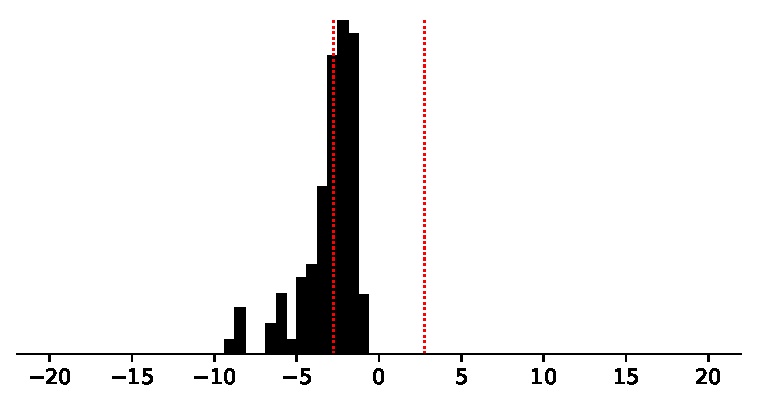
\includegraphics[width=.31\textwidth]{figures/sonar_0_7.eps}}\\
\midrule & \textsc{gnb} & \textsc{knn} & \textsc{t} & $p$ & \textsc{d}\\
$\approx$ &  0.681 & \bfseries 0.784 & -3.06 & 0.04 & ---\\
& {\tiny(0.07)} & {\tiny(0.06)} & & &\\\midrule
=         &  0.667 &  0.726 & -1.05 & 0.35 & 0.5418\\
  & {\tiny(0.07)} & {\tiny(0.06)} & &\\
-         &  0.653 & \bfseries 0.788 & -9.29 & 0.00 & 0.4582\\
  & {\tiny(0.07)} & {\tiny(0.06)} & &\\
+         & --- & --- & --- & --- & 0.0000\
\\&  & & & &\\\bottomrule
\end{tabularx}

%\hspace{.01\textwidth}
\end{table}

Therefore, the interpretation of the example table will be as follows. The average value of the observation indicates no predominance of any considered algorithm withe the accuracies of approximately 78\% for \textsc{knn} and 68\% for \textsc{gnb}. The average T-statistics value is -3.06, which gives \emph{p value} at 0.04, which makes it a statistically significant difference.

However, we may also observe situations in which a significant difference between algorithms does not occur (line $=$), where T-statistic equal -1.05, which gives \emph{p value} at 0.36. Similar situations (no significant difference) occurs in 54\% of the considered cases. Divisions which show a significant advantage of the \textsc{knn} algorithm occur in 46\% of cases, and the extreme value of T-statistics is -9.26, which is an outlier in the context of the problem under consideration.

In connection with the above observations, we can properly validate two contradictory research hypotheses by pulling the dataset into folds adequately many times. Moreover, with the average value of T-statistics close to the significance level, approximately a quarter of the experiments will give us information about the \textsc{knn} advantage, when all the other cases of the divisions will deny any statistical difference.

The simplest of situations encountered in performed experiments is that in which each of ten thousand experiments leads to the same conclusion, as is shown in the examples in the Table \ref{tab:single}. The distribution of T-statistics in such cases is either narrow enough to fit within the critical region (\textsc{soybean}) or far enough from it, so that even outlier observations leading to other conclusions do not happen. It is worth noting, however, that even in such cases, outliers reveal a major deviation from the mean value (for example, an average of 11.74 in the \textsc{wine} dataset and an outlier observation of 33.48). It is particularly important to note at this point that only twelve of the fifty-four comparisons are characterized by such unambiguous conclusions.

\begin{table}[!h]
	\centering
	\caption{Three example summaries of ten thousand repetitions of 5-fold cross-validation used to compare two classifiers using t test over accuracy score showing \textbf{results evident for one hypothesis}.}
	\label{tab:single}
	\scriptsize\begin{tabularx}{.31\textwidth}{@{\hspace{.5em}}c@{\hspace{.5em}}c@{\hspace{.5em}}c|CCC}
\toprule\multicolumn{6}{c}{\textsc{wine regular}}\\\bottomrule
\multicolumn{6}{@{}c@{}}{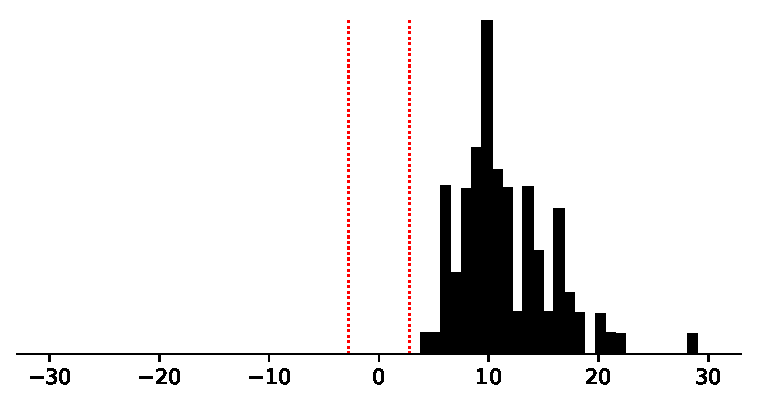
\includegraphics[width=.31\textwidth]{figures/wine_0_7.eps}}\\
\midrule & \textsc{gnb} & \textsc{knn} & \textsc{t} & $p$ & \textsc{d}\\
$\approx$ & \bfseries 0.974 &  0.690 & 11.74 & 0.00 & ---\\
& {\tiny(0.03)} & {\tiny(0.06)} & & &\\\midrule
-         & --- & --- & --- & --- & 0.0000\
\\&  & & & &\\
-         & --- & --- & --- & --- & 0.0000\
\\&  & & & &\\
+         & \bfseries 0.977 &  0.702 & 33.48 & 0.00 & 1.0000\\
  & {\tiny(0.03)} & {\tiny(0.06)} & &\\\bottomrule
\end{tabularx}\hspace{.03\textwidth}%
	\scriptsize\begin{tabularx}{.31\textwidth}{@{\hspace{.5em}}c@{\hspace{.5em}}c@{\hspace{.5em}}c|CCC}
\toprule\multicolumn{6}{c}{\textsc{soybean regular}}\\\bottomrule
\multicolumn{6}{@{}c@{}}{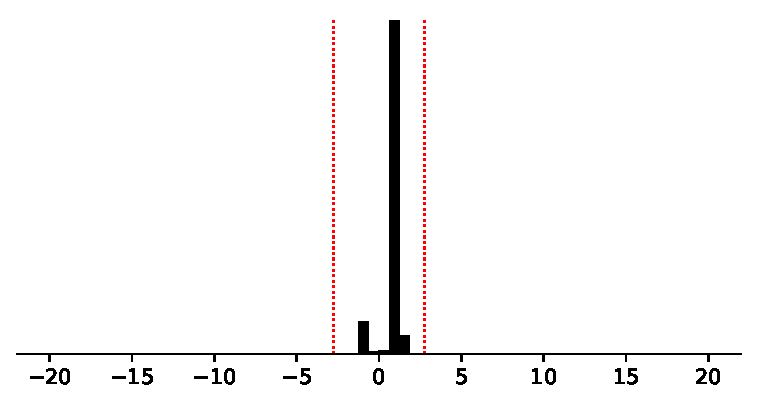
\includegraphics[width=.31\textwidth]{figures/soybean_1_7.eps}}\\
\midrule & \textsc{gnb} & \textsc{cart} & \textsc{t} & $p$ & \textsc{d}\\
$\approx$ &  0.998 &  0.989 & 0.87 & 0.43 & ---\\
& {\tiny(0.01)} & {\tiny(0.04)} & & &\\\midrule
=         &  0.978 &  0.978 & 0.00 & 1.00 & 0.4388\\
  & {\tiny(0.01)} & {\tiny(0.04)} & &\\
-         & --- & --- & --- & --- & 0.0000\
\\&  & & & &\\
+         & --- & --- & --- & --- & 0.0000\
\\&  & & & &\\\bottomrule
\end{tabularx}\hspace{.03\textwidth}%
	\scriptsize\begin{tabularx}{.31\textwidth}{@{\hspace{.5em}}c@{\hspace{.5em}}c@{\hspace{.5em}}c|CCC}
\toprule\multicolumn{6}{c}{\textsc{monkone regular}}\\\bottomrule
\multicolumn{6}{@{}c@{}}{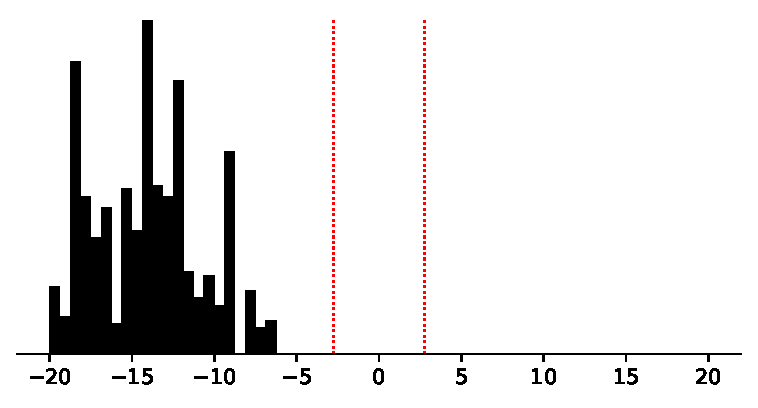
\includegraphics[width=.31\textwidth]{figures/monkone_0_7.eps}}\\
\midrule & \textsc{gnb} & \textsc{knn} & \textsc{t} & $p$ & \textsc{d}\\
$\approx$ &  0.664 & \bfseries 0.945 & -18.24 & 0.00 & ---\\
& {\tiny(0.04)} & {\tiny(0.02)} & & &\\\midrule
-         & --- & --- & --- & --- & 0.0000\
\\&  & & & &\\
-         &  0.664 & \bfseries 0.957 & -47.89 & 0.00 & 1.0000\\
  & {\tiny(0.04)} & {\tiny(0.02)} & &\\
+         & --- & --- & --- & --- & 0.0000\
\\&  & & & &\\\bottomrule
\end{tabularx}
\end{table}


The dominant majority, as many as 34 out of 54 comparisons correspond to the situation presented in the example in Table 1, where we can draw two contradictory conclusions from the appropriate (let's emphasize - random) combination of patterns division into folds. Examples here are presented in Table \ref{tab:double}. In the case of the \textsc{wine} dataset, we may observe a situation in which the \textsc{gnb} algorithm in averaging achieves an advantage over the \textsc{cart}, but in a quarter of the cases, random division of the dataset will lead to the conclusion that there are no significant differences. A much more interesting case is the \textsc{iris} dataset, where in 94\% of divisions there is no significant difference between the compared classifiers, but 2\% of the problem instances leads to the conclusion that the \textsc{knn} has a significant advantage over \textsc{gnb}. An even stronger example of this type is another case of the \textsc{wine} dataset, where, despite the predominance of the \textsc{dtc} over the \textsc{knn} and the average difference in quality at 21\%, we can still find one part-per-thousand of situations in which the statistical difference between them disappears.

\begin{table}[!h]
	\centering
	\caption{Three example summaries of ten thousand repetitions of 5-fold cross-validation used to compare two classifiers using t test over accuracy score showing results pointing \textbf{two different hypotheses}.}

	\label{tab:double}

	\scriptsize\begin{tabularx}{.31\textwidth}{@{\hspace{.5em}}c@{\hspace{.5em}}c@{\hspace{.5em}}c|CCC}
\toprule\multicolumn{6}{c}{\textsc{wine regular}}\\\bottomrule
\multicolumn{6}{@{}c@{}}{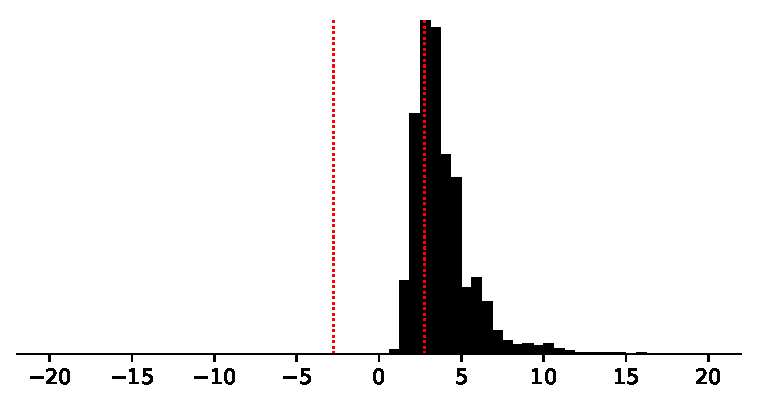
\includegraphics[width=.31\textwidth]{figures/wine_1_7.eps}}\\
\midrule & \textsc{gnb} & \textsc{cart} & \textsc{t} & $p$ & \textsc{d}\\
$\approx$ & \bfseries 0.974 &  0.905 & 3.91 & 0.02 & ---\\
& {\tiny(0.03)} & {\tiny(0.05)} & & &\\\midrule
=         &  0.967 &  0.961 & 0.32 & 0.76 & 0.2751\\
  & {\tiny(0.03)} & {\tiny(0.05)} & &\\
-         & --- & --- & --- & --- & 0.0000\
\\&  & & & &\\
+         & \bfseries 0.972 &  0.944 & 69.20 & 0.00 & 0.7249\\
  & {\tiny(0.03)} & {\tiny(0.05)} & &\\\bottomrule
\end{tabularx}\hspace{.03\textwidth}%
	\scriptsize\begin{tabularx}{.31\textwidth}{@{\hspace{.5em}}c@{\hspace{.5em}}c@{\hspace{.5em}}c|CCC}
\toprule\multicolumn{6}{c}{\textsc{iris regular}}\\\bottomrule
\multicolumn{6}{@{}c@{}}{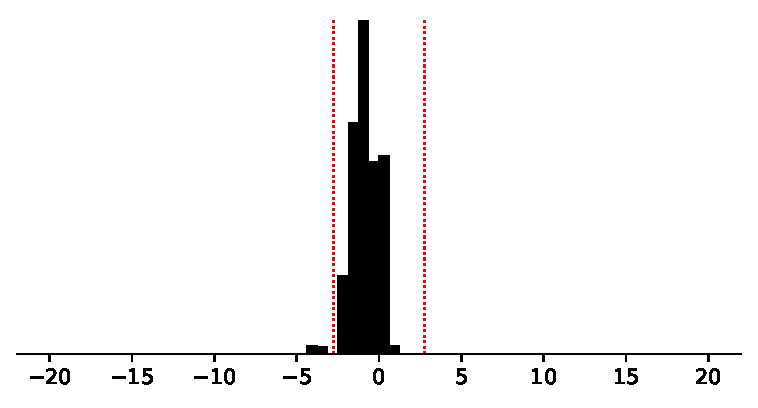
\includegraphics[width=.31\textwidth]{figures/iris_0_7.eps}}\\
\midrule & \textsc{gnb} & \textsc{knn} & \textsc{t} & $p$ & \textsc{d}\\
$\approx$ &  0.954 &  0.965 & -1.00 & 0.37 & ---\\
& {\tiny(0.03)} & {\tiny(0.03)} & & &\\\midrule
=         &  0.960 &  0.960 & 0.00 & 1.00 & 0.9389\\
  & {\tiny(0.03)} & {\tiny(0.03)} & &\\
-         &  0.947 & \bfseries 0.973 & -4.00 & 0.02 & 0.0204\\
  & {\tiny(0.03)} & {\tiny(0.03)} & &\\
+         & --- & --- & --- & --- & 0.0000\
\\&  & & & &\\\bottomrule
\end{tabularx}\hspace{.03\textwidth}%
	\scriptsize\begin{tabularx}{.31\textwidth}{@{\hspace{.5em}}c@{\hspace{.5em}}c@{\hspace{.5em}}c|CCC}
\toprule\multicolumn{6}{c}{\textsc{wine regular}}\\\bottomrule
\multicolumn{6}{@{}c@{}}{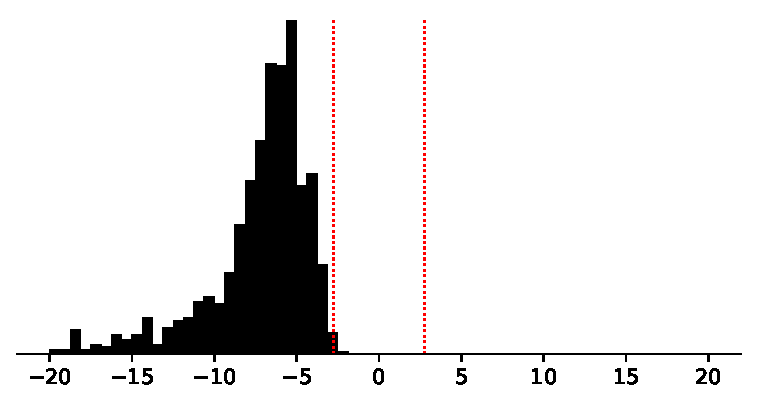
\includegraphics[width=.31\textwidth]{figures/wine_2_7.eps}}\\
\midrule & \textsc{knn} & \textsc{cart} & \textsc{t} & $p$ & \textsc{d}\\
$\approx$ &  0.690 & \bfseries 0.905 & -7.48 & 0.00 & ---\\
& {\tiny(0.06)} & {\tiny(0.05)} & & &\\\midrule
=         &  0.724 &  0.847 & -2.30 & 0.08 & 0.0011\\
  & {\tiny(0.06)} & {\tiny(0.05)} & &\\
-         &  0.702 & \bfseries 0.921 & -57.30 & 0.00 & 0.9989\\
  & {\tiny(0.06)} & {\tiny(0.05)} & &\\
+         & --- & --- & --- & --- & 0.0000\
\\&  & & & &\\\bottomrule
\end{tabularx}
\end{table}

The most interesting, however, is the third, last group of observations, which consists of 8 out of 54 examples (Table \ref{tab:triple}). There is a set of cases in which, depending on which of the random dataset divisions we select for the experiment, we may get the validation of each possible conclusion. The liver dataset is particularly interesting here, where only 3 out of 100 000 cases show the \textsc{cart} algorithm superiority over \textsc{knn}, with approximately 94\% of their equal quality and 5\% of \textsc{knn} advantage cases.

This may lead to the hypothesis that if we have the sufficiently large computational power to repeat random dataset divisions, we will lead to a situation in which, using the standard approach to experiments, we will be able to reasonably support any hypothesis about the statistical relationship between the compared classifiers. Moreover, based on all separate groups of cases, we can undoubtedly conclude that the existence of such combinations of data sets and classification algorithms is common, against which we can support contradictory hypotheses, depending on the applied random division of the data set into folds.

\begin{table}[!h]
	\centering

	\caption{Three example summaries of ten thousand repetitions of 5-fold cross-validation used to compare two classifiers using t test over accuracy score showing results pointing \textbf{all the possible hypotheses}.}

	\label{tab:triple}
	\scriptsize\begin{tabularx}{.31\textwidth}{@{\hspace{.5em}}c@{\hspace{.5em}}c@{\hspace{.5em}}c|CCC}
\toprule\multicolumn{6}{c}{\textsc{liver regular}}\\\bottomrule
\multicolumn{6}{@{}c@{}}{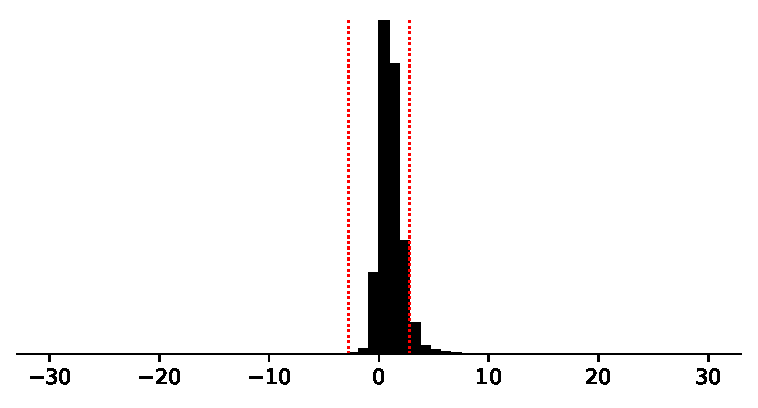
\includegraphics[width=.31\textwidth]{figures/liver_2_7.eps}}\\
\midrule & \textsc{knn} & \textsc{cart} & \textsc{t} & $p$ & \textsc{d}\\
$\approx$ & \bfseries 0.663 &  0.634 & 26095085296.29 & 0.00 & ---\\
& {\tiny(0.05)} & {\tiny(0.05)} & & &\\\midrule
=         &  0.643 &  0.643 & 0.00 & 1.00 & 0.9413\\
  & {\tiny(0.05)} & {\tiny(0.05)} & &\\
-         &  0.638 & \bfseries 0.655 & -6.00 & 0.00 & 0.0003\\
  & {\tiny(0.05)} & {\tiny(0.05)} & &\\
+         & \bfseries 0.699 &  0.641 & 2609508529517727.50 & 0.00 & 0.0584\\
  & {\tiny(0.05)} & {\tiny(0.05)} & &\\\bottomrule
\end{tabularx}\hspace{.03\textwidth}%
	\scriptsize\begin{tabularx}{.31\textwidth}{@{\hspace{.5em}}c@{\hspace{.5em}}c@{\hspace{.5em}}c|CCC}
\toprule\multicolumn{6}{c}{\textsc{german regular}}\\\bottomrule
\multicolumn{6}{@{}c@{}}{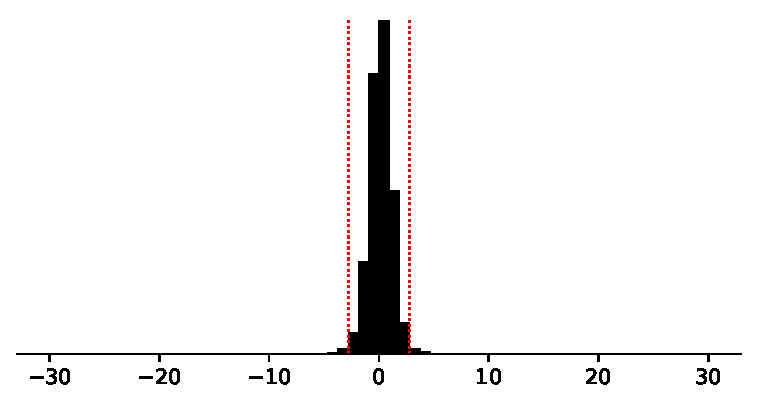
\includegraphics[width=.31\textwidth]{figures/german_2_7.eps}}\\
\midrule & \textsc{knn} & \textsc{cart} & \textsc{t} & $p$ & \textsc{d}\\
$\approx$ &  0.691 &  0.688 & 0.15 & 0.89 & ---\\
& {\tiny(0.02)} & {\tiny(0.03)} & & &\\\midrule
=         &  0.688 &  0.688 & 0.00 & 1.00 & 0.9807\\
  & {\tiny(0.02)} & {\tiny(0.03)} & &\\
-         &  0.693 & \bfseries 0.709 & -16.00 & 0.00 & 0.0096\\
  & {\tiny(0.02)} & {\tiny(0.03)} & &\\
+         & \bfseries 0.712 &  0.682 & 18.97 & 0.00 & 0.0097\\
  & {\tiny(0.02)} & {\tiny(0.03)} & &\\\bottomrule
\end{tabularx}\hspace{.03\textwidth}%
	\scriptsize\begin{tabularx}{.31\textwidth}{@{\hspace{.5em}}c@{\hspace{.5em}}c@{\hspace{.5em}}c|CCC}
\toprule\multicolumn{6}{c}{\textsc{diabetes regular}}\\\bottomrule
\multicolumn{6}{@{}c@{}}{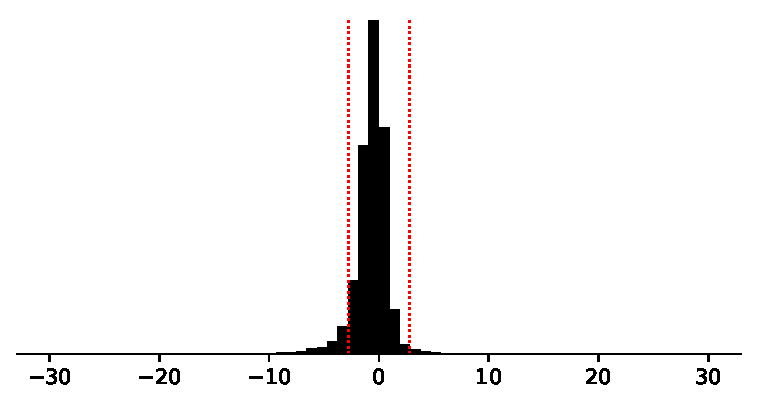
\includegraphics[width=.31\textwidth]{figures/diabetes_2_7.eps}}\\
\midrule & \textsc{knn} & \textsc{cart} & \textsc{t} & $p$ & \textsc{d}\\
$\approx$ &  0.691 &  0.701 & -0.67 & 0.54 & ---\\
& {\tiny(0.03)} & {\tiny(0.04)} & & &\\\midrule
=         &  0.682 &  0.682 & 0.00 & 1.00 & 0.9286\\
  & {\tiny(0.03)} & {\tiny(0.04)} & &\\
-         &  0.681 & \bfseries 0.716 & -21.90 & 0.00 & 0.0610\\
  & {\tiny(0.03)} & {\tiny(0.04)} & &\\
+         & \bfseries 0.714 &  0.677 & 11.06 & 0.00 & 0.0104\\
  & {\tiny(0.03)} & {\tiny(0.04)} & &\\\bottomrule
\end{tabularx}
\end{table}

\begin{table}[!h]
	\centering
	\caption{ABCD}\vspace{.5em}
	\label{tab:comparison}
	\begin{tabularx}{.5\textwidth}{lCCC}
		\toprule
		\bfseries \textsc{test used} & \multicolumn{3}{c}{\bfseries\textsc{number of supported hypotheses}}\\
		& \bfseries \textsc{i} & \bfseries \textsc{ii} & \bfseries \textsc{iii}\\\midrule
		\emph{without correction} & 12 & 34 &  8 \\
		\emph{parametric (corr=.1)} & 11 & 35 &  8 \\
		\emph{parametric (corr=.2)} & 11 & 35 &  8 \\
		\emph{parametric (corr=.3)} &  9 & 39 &  6 \\
		\emph{parametric (corr=.4)} &  9 & 39 &  6 \\
		\emph{parametric (corr=.5)} &  9 & 39 &  6 \\
		\emph{parametric (corr=.6)} & 13 & 36 &  5 \\
		\emph{non-parametric} & 23 & 31 &  0 \\
		\bottomrule
	\end{tabularx}
\end{table}

\end{document}
